
\chapter{Memoria} % Título del capítulo

\label{Memoria} % etiqueta \ref{Memoria}

\section{Introducción}

Atendiendo al contexto socioeconómico actual es razonable señalar que el conjunto de conocimientos, tanto teóricos como tecnológicos, asociados al desarrollo de la IA (Inteligencia Artificial) suponen un ámbito científico estratégico. 
En este sentido, la investigación actúa como herramienta vertebradora de su progreso. 
De esta manera, se faculta a los ingenieros/as para materializar y perfeccionar las innovaciones que definirán su evolución. 

En términos generales, la IA está basada en modelos de redes neuronales.
Existen varias formas de enfocar la gestión computacional de estos modelos.
La tendencia general es emplear unidades de procesamiento gráfico en combinación con procesadores complejos administrados por sistemas operativos. 
De este modo, se consigue gestionar grandes volúmenes de datos, lo que conlleva un entrenamiento óptimo y en consecuencia un aprendizaje exitoso.
No obstante, la infraestructura necesaria para tal fin ocupa un tamaño considerable.
Además, se requiere de una gran cantidad de energía.
Hay ocasiones en las que el tamaño y/o la potencia consumida son factores determinantes, por ejemplo, en unidades autónomas con capacidad de operar aisladas como satélites, vehículos autónomos etc.
En estos casos la IA es necesaria para el desempeño de sus funciones, pero su procesamiento debe estar descentralizado en su propio hardware.
Este procesamiento de algoritmos de \textit{Machine Learning} a nivel local y sin necesidad de estar conectados a internet es lo que se conoce como IA en el borde \cite{IA-edge} (\textit{AI at the edge}) y surge en contraposición a los modelos conectados a la nube.
Además, cabe destacar que realizar por completo el creciente número de procesos de IA en la nube no sólo no es deseable, sino que es insostenible \cite{Efficient-Inference}. 
% Machine Learning -> aprendizaje máquina

Para llevar a cabo la inferencia de IA en el borde, se sugiere un enfoque de gestión computacional distribuido.
A este respecto, se plantea el uso de FPGAs.
Se propone implementar en estos dispositivos una arquitectura SoC heterogénea con un microcontrolador acoplado a coprocesadores de aplicación específica.
De esta manera, se consigue distribuir las tareas con objeto de ganar flexibilidad y lograr una mayor eficiencia.
Por un lado, el microcontrolador permite programabilidad y capacidad de gestionar los datos de entrada/salida. 
Por otro lado, los coprocesadores embebidos permiten realizar las operaciones asociadas a las redes neuronales con un alto rendimiento. 
Existen varios modos de acoplar estos dos tipos de diseños.
A lo largo del desarrollo de este trabajo se realiza una caracterización del rendimiento de los diferentes modos de conexión que ofrece el microcontrolador RISC-V seleccionado.
Mediante esta caracterización se pretende concluir el método de acoplamiento más adecuado en términos de latencia.
Como se ha mencionado, la sugerencia de distribución computacional para llevar a cabo IA en el borde conlleva externalizar los cálculos asociados a las redes neuronales del micro a coprocesadores embebidos.
En lo referente a este trabajo, se comienza por evaluar un acelerador relativo al cálculo de funciones de activación, particularmente la función sigmoide.
%Se escoge está función ya que al contener exponenciales su cálculo supone numerosos ciclos de reloj si se efectúan íntegramente mediante un microcontrolador. 
Se escoge está función ya que requiere de operaciones matemáticas que no son directas para la ALU.
Esto le supone al micro numerosos ciclos de reloj para calcularla. 
Por lo tanto, emplear un coprocesador embebido para acelerar este proceso resulta en un ahorro significativo del tiempo de computación.
Este acelerador se integra al microcontrolador seleccionado mediante el método previamente determinado como el más adecuado. 
Finalmente, se corroboran los beneficios de emplear este tipo de enfoque distribuido.

La investigación presentada en este trabajo ha sido desarrollada en el Grupo de Investigación de Diseño en Electrónica Digital (GDED) y se ha realizado en el marco de unas practicas remuneradas de 5 meses de duración.
El grupo está familiarizado con el diseño hardware, así como con su descripción empleando principalmente el lenguaje VHDL. 
Asimismo, fomenta el uso de herramientas FLOS, así como la metodología de integración continua (CI), que en conjunción con programas/plataformas de control de versiones, han sido esenciales para la gestión eficaz de todo el código empleado.
En definitiva, la colaboración con el grupo ha sido determinante para la correcta realización de este Trabajo Fin de Máster.

\section{Contexto}

%Aquí irá el contexto. ISA libres RISC-V. \textit{} \textbf{} \underline{}
El primer paso para llevar a cabo este proyecto es realizar la selección del microcontrolador.
Se requiere de su implementación en FPGA, por lo que se necesita la descripción en HDL de su arquitectura.
Es interesante destacar que el término empleado para referirse a este formato es \textit{soft-core} (núcleo blando).
A diferencia de los micros \textit{hard-core} (núcleo duro), es decir, los impresos en silicio, los \textit{soft-cores} están pensados para ser implementados en dispositivos lógicos programables. 
%puede que retocar
Además, no solo se precisa de la descripción hardware del micro sino también de las herramientas asociadas para compilar software interpretable por el mismo.
En este sentido, la búsqueda se ha centrado en un proyecto \textit{royalty-free} (libre de derechos).

%verbos!!!

El siguiente paso es evaluar los diferentes modos de acoplamiento de coprocesadores con los que cuenta el micro seleccionado.
Con objeto de caracterizar el rendimiento de cada uno de ellos y concretar el más adecuado para nuestro propósito.
Para ello, se testean varios aceleradores acoplados al micro mediante todos los modos de los que este dispone.
De esta manera, se obtiene un conjunto de bancos de prueba para ensayar en simulación y así proporcionar las lecturas de latencia y throughput de cada uno de los métodos de conexión.
En concreto, se han acoplado 3 multiplicadores con diferentes características.
Además, todos los ensayos se han implementados en FPGA para verificar su correcta operatividad.

El último paso es comenzar a abordar un enfoque distribuido para realizar IA en el borde. 
A este respecto, se requiere de aceleradores embebidos que realicen los cálculos asociados a las redes neuronales.
Atendiendo a la caracterización realizada en el paso anterior, se establece un criterio mediante el cual decidir que modo de conexión emplear para acoplar estos diseños embebidos.
Una vez acoplados, se corrobora el beneficio de utilizar coprocesadores frente a realizar los cálculos íntegramente mediante las funcionalidades del micro.
Para ello, se realiza un banco de pruebas que compare en simulación los ciclos de ejecución de ambos planteamientos.
Dado el limitado tiempo de investigación tan solo se ha externalizado el cálculo de la activación a través de la función sigmoide.
Para lo cual, se ha utilizado un acelerador embebido diseñado por Koldo Basterretxea.

\subsection{ISAs libres}

\label{isas-free}

%explicación ISA
A grandes rasgos, la CPU o núcleo del microcontrolador, es la unidad encargada de decodificar y ejecutar secuencialmente las instrucciones que previamente extrae de un programa almacenado en memoria.
%Previamente? secuencial donde ponerlo
Estas instrucciones codifican operaciones y dependen de la arquitectura que las procesa para aplicarlas.
En otras palabras, el mecanismo secuencial de extracción/decodificación/ejecución de instrucciones transforma sucesivamente una operación (aritmeticológica, de movimiento de datos etc.) de un plano conceptual, codificada en un programa, a un plano material, es decir, físicamente haciendo uso de los recursos electrónicos de la arquitectura digital. 
Es por ello que el set de instrucciones está íntimamente ligado a la arquitectura y definirlo condiciona de manera abstracta la topología de la misma. 
En este sentido, una arquitectura de conjunto de instrucciones (ISA) es una especificación de instrucciones que permite generar arquitecturas de procesadores a partir de ella.
Además, este concepto debe estar complementado con un soporte para compilar lenguajes de alto nivel, como por ejemplo C, que mediante las herramientas y librerías necesarias traduzcan su sintaxis a instrucciones para una ISA en concreto.

%Estos tres recursos, arquitectura digital, ISA y herramientas para compilar forman un proyecto de microcontrolador.

En el siglo pasado, el desarrollo de microarquitecturas estaba completamente monopolizado por el ámbito privado.
Esto se debía a que el esfuerzo de definir una ISA y dar soporte para la compilación de su set de instrucciones, además de verificar todo su ecosistema, era demasiado elevado para afrontarlo desde un punto de vista \textit{Open Source} (código abierto).
Es por ello que a comienzos del siglo XXI eran pocos los proyectos de hardware libre de este tipo.
Caben mencionar los procesadores OpenRISC \cite{openrisc} basados en su propia ISA y desarrollados por la comunidad OpenCores \cite{opencores} y los procesadores OpenSPARC \cite{opensparc} y LEON \cite{leon} (proyecto referente de la ESA), basados en la ISA SPARC.
No obstante, entre mediados de los 2000 y de la década de 2010, han aumentado las especificaciones de ISAs libres de derechos que se han puesto a disposición de los usuarios.
Esto se ha debido principalmente a tres motivos.
El primero de ellos es porque las patentes han expirado.
Este es el caso de la ISA SuperH \cite{superh}.
Durante la crisis económica asiática de 1997 Hitachi se asoció con Mitsubishi y escindió su división de microcontroladores en una nueva compañía llamada Renesas \cite{new-comp}.
Esta compañía no heredó los ingenieros de Hitachi que habían desarrollado SuperH, por lo que con el tiempo Renesas perdió el interés por ella y expiraron sus patentes.
Un ejemplo de diseño de código abierto que utiliza este set de instrucciones es el procesador J-core \cite{j-core}.
El segundo motivo es porque se han dado las circunstancias materiales necesarias para llevar a cabo un proyecto de ISA abierto concebido desde el primer momento como \textit{Open Source}.
Este es el caso de RISC-V \cite{waterman13}.
El tercer motivo es porque a consecuencia de la enorme relevancia del proyecto anterior, las compañías intencionalmente han decidido abrir las especificaciones. 
Este es el caso de POWER ISA \cite{power}.
A principios de la década de 1990, IBM desarrolló una ISA llamada IBM POWER (\textit{Performance Optimization With Enhanced RISC}) para la familia de procesadores POWER.
Más tarde, a finales de los 90, esta arquitectura se abandonó y lo que se había convertido en PowerPC evolucionó hasta que en 2006 se estableció como POWER ISA. 
En 2019, IBM decidió hacer esta ISA \textit{Open Source} y desde entonces es mantenida por la fundación OpenPower \cite{open-power}.
Tres ejemplos de diseños de código abierto que utilizan este set de instrucciones son Microwatt \cite {gh:microwatt}, Chiselwatt \cite{gh:chiselwatt} y Libre-SOC \cite{libre-soc}.

\subsection{Ecosistema RISC-V}

\label{eco-risc}

En mayo de 2010, como parte del Laboratorio de Computación Paralela (Par Lab) de la universidad de Berkeley, el profesor Krste Asanović y los estudiantes de posgrado Yunsup Lee y Andrew Waterman iniciaron la especificación de un set de instrucciones denominado RISC-V.
El Par Lab fue un proyecto dirigido por David Patterson y subvencionado con capital privado proveniente de empresas como Intel y Microsoft, además de con fondos públicos del estado de California.
Cabe destacar que todos los proyectos del Par Lab eran de código abierto y utilizaban la licencia \textit{Berkeley Software Distribution} (BSD), incluido RISC-V.
El 13 de mayo de 2011 se publicó el primer manual del set de instrucciones de RISC-V bajo el nombre \textit{The RISC-V Instruction Set Manual, Volume I: Base User-Level ISA} \cite{manual-riscv}.
Ese mismo año se realizó el primer \textit{tapeout} de un chip RISC-V, producido en 28nm.
Durante los siguientes años se realizaron publicaciones y talleres.
A este respecto, una publicación interesante es la realizada en 2014 por Asanović y Patterson titulada \textit{Instruction Sets Should Be Free: The Case For RISC-V} \cite{paper-riscv} donde se plantean argumentos que defienden una ISA libre y abierta. 
En concreto, RISC-V pasó a ser de dominio público en el momento en el que se publicaron los informes técnicos que definen la ISA, aunque el texto de dichos informes está bajo una licencia de \textit{Creative Commons} para permitir su mejora por colaboradores externos.
Además, no se ha registrado ninguna patente relativa a RISC-V, puesto que esta ISA per se no representa ninguna tecnología novedosa.
En 2015, se creó la fundación RISC-V con el objetivo de construir una comunidad abierta e internacionalizar el proyecto.
En 2018 la fundación RISC-V anunció una colaboración conjunta con la Fundación Linux en términos de cooperación técnica y estratégica, lo que incluye apoyo operativo, gestión de miembros, contabilidad, divulgación comunitaria etc. 
En marzo de 2020, la Asociación Internacional RISC-V se constituyó en Suiza debido a factores geopolíticos externos que defienden la continuidad del modelo de propiedad intelectual.
El interés de la Asociación Internacional RISC-V es animar a organizaciones, particulares y entusiastas a hacer posible una nueva era de innovación en procesadores a través de la colaboración en estándares abiertos y \textit{Open Source}.

En este sentido, las plataformas de control de versiones, como GitHub y GitLab, cumplen un papel crucial a la hora de compartir entre los usuarios sus diseños de núcleos y microcontroladores SoC basados en esta ISA libre.
En particular, el primer proyecto de un procesador RISC-V se escribió en Chisel \cite{bachrach:2012:chisel}.
No obstante, en la actualidad hay multitud de proyectos en todo tipo de lenguajes de descripción de hardware.
Existe una lista de implementaciones RISC-V de código abierto \cite{marchid} donde se pueden consultar los proyectos \textit{Open Source} más relevantes.
Además, a cada uno de ellos se le asigna un identificador (ID).
Algunos de estos ejemplos son:

\begin{itemize}
    \item En Scala:
        \begin{itemize}
            \item Rocket Chip \cite{gh:rocket-chip} ID: 1
            \item VexRiscv \cite{gh:VexRiscv} ID: 33
        \end{itemize}
    \item En Verilog:
        \begin{itemize}
            \item PicoRV32 \cite{gh:picorv32} ID: none \footnote{A pesar de no tener ID se considera un proyecto \textit{Open Source} de gran relevancia.}
            \item Hummingbirdv2 E203 \cite{gh:e203-hbirdv2} ID: 26
            \item Steel Core \cite{gh:riscv-steel} ID: 24
            \item SERV \cite{gh:serv} ID: 18
        \end{itemize}
    \item En VHDL:
        \begin{itemize}
            \item NEORV32 \cite{gh:neorv32} ID: 19
            \item ORCA \cite{gh:ORCA-risc-v} ID: 7
            %\item Potato \cite{gh:potato} ID: none
        \end{itemize}
\end{itemize} 

\subsubsection{CFUs/CXUs}

Una de las finalidades de este proyecto de investigación es realizar una caracterización del rendimiento de los métodos de acoplamiento de coprocesadores en núcleos RISC-V.
A este respecto, un procesador basado en RISC-V no solo se limita a ofrecer la posibilidad de dar soporte para conexiones mapeadas en memoria o comunicaciones mediante interfaces \textit{stream}.
Un concepto destacable que posibilitan los núcleos basados en esta ISA es el de gestionar instrucciones personalizadas (\textit{custom}).
Haciendo uso de este concepto surge la oportunidad de realizar extensiones de instrucciones personalizadas y asociarlas con aceleradores embebidos.
%puede que retocar-Hecho!
Esta vinculación resulta muy ventajosa, ya que permite a la CPU resolver aplicaciones especificas decodificando instrucciones \textit{custom}.
De esta modo, se deriva la información directamente al acelerador embebido de manera similar a como lo haría una instrucción de suma con la ALU. 
Es decir, se consigue una integración completa del acelerador dentro del \textit{pipeline} de la CPU, lo que significa una forma muy eficiente de acoplar micro y coprocesador.
A priori, lo que resulta como una ventaja evidente puede conllevar algunos inconvenientes.
%Comas aqui?-Retocado!
Esto es debido a que las librerías de software que utilizan estas extensiones y los núcleos que las implementan son creados por diferentes organizaciones.
Comúnmente estas utilizan herramientas diferentes y sus desarrollos, aunque aislados son operativos, al integrarlos para genera un nuevo sistema podrían no funcionar.
Es por ello que se requiere de cierta estandarización que permita la reutilización robusta de las extensiones y librerías, además de proporcionar un modelo de programación uniforme para todas ellas.

En este sentido, en 2019, Google propuso el concepto \textit{Custom Function Unit} (CFU) \cite{prakash23} y lo integró en la CPU VexRiscv.
A partir de entonces esta extensión ha ganado popularidad y otras microarquitecturas RISC-V han añadido esta funcionalidad.
Derivado de este trabajo, existe un borrador que especifica la integración hardware-software de estas unidades de funcionalidades personalizadas \cite{CFU-draft}. 
En este texto se propone el concepto de \textit{Composable eXtension Unit} (CXU), que sería análogo al concepto de CFU. 
%Y se anima a cualquiera a definir, desarrollar y usar CXUs y sus librerías CX con el objetivo de que coexistan un número ilimitado de ellas desarrolladas de forma independiente dentro de una ISA fija y mediante un método de multiplexación conseguir la funcionalidad del conjunto.

%nexo con neorv32

\subsection{NEORV32}

\label{neorv32}

%foto opcode cfu
    
El NEORV32 es un microcontrolador SoC personalizable \textit{Open Source} construido entorno a la CPU RISC-V homónima NEORV32.
El repositorio principal del proyecto comenzó el 23 de junio de 2020 con un primer \textit{commit} de su creador y máximo contribuidor Stephan Nolting.

Para la elaboración de este proyecto de investigación resulta de gran importancia conocer los métodos de conexión disponibles en el NEORV32.
A este respecto, los principales modos de acoplamiento de coprocesadores con los que cuenta este microcontrolador son los siguientes:

\begin{itemize}
    \item \textit{Stream Link Interface} (SLINK)
    \item \textit{Processor-External Bus Interface} (XBUS)
    \item \textit{Custom Functions Subsystem} (CFS)
    \item \textit{Custom Functions Unit} (CFU)
\end{itemize} 

Se procede a hacer un breve descripción de cada uno de ellos.
En primer lugar, \textit{Stream Link} es una interfaz para realizar transmisiones \textit{stream} compatible con un subconjunto de AXI4-Stream \cite{axi}.
Esta interfaz proporciona canales RX y TX unidireccionales e independientes para enviar y recibir un flujo de datos.
Cada canal dispone de una FIFO interna configurable para almacenar los datos provenientes del \textit{stream}.
En segundo lugar, \textit{Processor-External Bus} es una interfaz de bus general para acoplar aceleradores mapeados en memoria compatible con Wishbone \cite{wb} y AXI4-Lite \cite{axi-lite}.
Esta interfaz cuenta con un módulo de caché opcional denominado \textit{X-CACHE}.
En tercer lugar, \textit{Custom Functions Subsystem} es un \textit{template} vacío que proporciona hasta 64 registros de lectura/escritura de 32 bits mapeados en memoria a los que la CPU puede acceder mediante operaciones normales de carga/almacenamiento.
En cuarto lugar, \textit{Custom Functions Unit} es una unidad funcional que se integra directamente en el \textit{pipeline} de la CPU.
Fue añadida al NEORV32 basándose en el borrador de la especificación CFU/CXU.
Esto permitió implementar instrucciones RISC-V personalizadas. 
Los formatos de instrucción soportados por el NEORV32 son \textit{R3-Type}, \textit{R4-Type} y \textit{R5-Type} \footnote{Cabe destacar que recientemente Stephan a eliminado el soporte para la instrucción \textit{R5-Type} \href{https://github.com/stnolting/neorv32/pull/971}{\#971}}.
Los dos primeros formatos son un estándar de RISC-V y el último es exclusivo de NEORV32. 
En concreto, el primer y el segundo formato permiten direccionar dos y tres registros de entrada de 32 bits, respectivamente. 
Además, la función se seleccionada a través de \textit{funct7} y/o \textit{funct3} en el primer caso y a través de \textit{funct3} en el segundo caso. 
El tercer formato permite direccionar cuatro registros de entrada de 32 bits. 
Al no disponer del campo \textit{funct3} y/o \textit{funct7} solo se pueden realizar dos funciones personalizadas a través de este formato, \textit{A format} y \textit{B format}.  
La figura \ref{fig:ins} muestra los tipos de instrucciones personalizadas de 32 bits soportadas por NEORV32 a través de la extensión ISA específica Zxcfu.

\begin{figure}[h!]
    \centering
    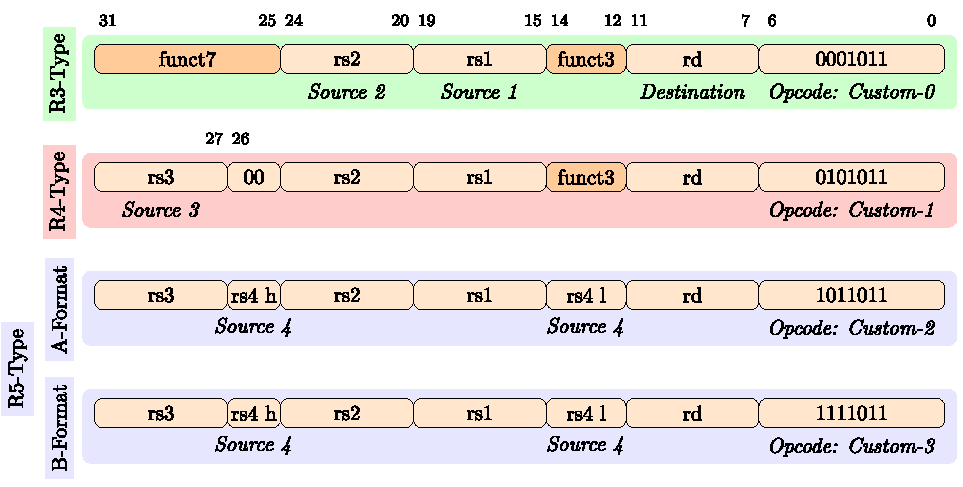
\includegraphics[width=14cm]{Figuras/CFU_INS.pdf}
    \caption{Tipos de instrucciones CFU \textit{custom} para el caso del NEORV32.}
    \label{fig:ins}
\end{figure}

A lo largo de estos cuatro años el proyecto ha estado en constante evolución.
A este respecto, son destacables las contribuciones que realizó el miembro de GDED Unai Martinez Corral (\textit{umarcor}) a lo largo del 2021 y 2022 entorno al tema de la integración continua del proyecto, además de llevar acabo su sugerencia de separar del repositorio principal el repositorio \textit{neorv32-setups}.
%mas cosas k no solapen con el punto 2.1 
En el transcurso del desempeño de este proyecto de investigación, se han visto aplicar numerosos cambios.
Con respecto a los modos de conexión se destacan las siguientes actualizaciones:
añadir a la interfaz SLINK la señal AXI-stream-compatible \textit{tlast} \href{https://github.com/stnolting/neorv32/pull/815}{\#815}, renombrar la interfaz de bus externa de \textit{Processor-External Memory Interface (WISHBONE)} a \textit{Processor-External Bus Interface (XBUS)} \href{https://github.com/stnolting/neorv32/pull/846}{\#846}, reajustar la interfaz CFU \href{https://github.com/stnolting/neorv32/pull/932}{\#932}.
Estas actualizaciones ejemplifican la constante transformación del proyecto. 
En el apartado \ref{Selec} se detallan los argumentos por los que se ha escogido este microcontrolador.

\subsection{CRI}

\label{cri}

Desde finales del siglo pasado, investigadores de multitud de universidades, incluyendo la universidad del País Vasco, han indagado sobre la posibilidad de externalizar cálculos, de procesadores de propósito general a aceleradores hardware específicos.
En 1999, el profesor Koldo Basterretxea, presentó un nuevo método recursivo para la aproximación de funciones basado en el uso de operadores reticulares modificados (MLO) \cite{basterretxea1999pwl} \cite{tarela2002optimised}.
El objetivo era utilizar este método como un marco general para realizar futuras implementaciones, especialmente enfocadas a los sistemas difusos (\textit{fuzzy}), así como a las redes neuronales artificiales (RNA).
Este método, denominado Centred Recursive Interpolation (CRI), es un algoritmo que opera nuevas funciones afines de interpolación a cada nivel de recursión.
Para hacerlo de manera sencilla y tratar de minimizar los parámetros del algoritmo, CRI genera funciones de interpolación centradas.

\begin{equation}\label{ec:1}
h_{1} = \frac{1}{2} (y_{1} + y_{2} - \Delta)\tag{*}
\end{equation}

Atendiendo a la ecuación \eqref{ec:1} encontramos el parámetro $\Delta$, denominado profundidad de interpolación.
CRI utiliza valores de $\Delta$ optimizados en cada nivel de recursión, de manera que se minimiza el error máximo de la aproximación.
En este sentido, para la aproximación mediante CRI de funciones paramétricas (con pendiente y saturación ajustable), se demuestra que el $\Delta$ optimizado es constante cuando variamos la pendiente.
Para el caso de la función paramétrica sigmoide \eqref{ec:2}, el $\Delta$ optimizado toma los siguientes valores para las 3 primeras recursiones:

\begin{table}[h!]
\centering
\caption{Tres primeras recursiones del $\Delta$opt (función sigmoide).}
\label{tab:1}
\begin{tabular}{|c|c|}
\hline
Sigmoide & $\Delta$opt    \\ \hline
q=1      & 0.3091 \\ \hline
q=2      & 0.2811 \\ \hline
q=3      & 0.2654 \\ \hline
\end{tabular}
\end{table}

\begin{equation}\label{ec:2}
\sigma(x)= \frac{1}{1 + e^{-x}}\tag{**}
\end{equation}

Desde un punto de vista hardware, Basterretxea ha realizao descripciones de diseños empleando este algoritmo desde el inicio de su planteamiento teórico.
A este respecto, en el repositorio del grupo de investigación, hay disponible un acelerador configurable y programable de funciones de activación basado en CRI.
Dicho acelerador soporta 7 tipos de FAs: sigmoide, tangente, lineal, ReLu, Hardlimit, satlin y leakyReLu. 
Para el presente trabajo de investigación, se ha utilizado exclusivamente la lógica referente a la función sigmoide.

\section{Anteproyecto}

\label{antepro}

%practicas no remuneradas
Como se ha mencionado, este proyecto se ha desempeñado en el marco de unas prácticas remuneradas tituladas \textit{Desarrollo de Custom Functional Units de IA para RISC-V}.
La duración de estas prácticas ha sido de 5 meses (594 horas) y por realizarlas se ha recibido una bolsa de ayuda total de 2000€.
No obstante, previas a estas prácticas remuneradas, se realizaron otras prácticas obligatorias relativas al \textit{practicum} del Máster.
Estas también se llevaron a cabo en el grupo de investigación GDED bajo el título \textit{Diseño e integración de CFU para RISC-V en FPGA}.
Tuvieron una duración de 2 meses y 20 días (225 horas) y fueron calificadas con una matrícula de honor (10).
Las tareas a desarrollar fueron las siguientes:

\begin{itemize}
    \item Realizar un \textit{set-up} de herramientas FOSS (\textit{Free and Open-Source Software}) para la implementación y simulación del proyecto.
%meter FOSS en acrónimos
    \item Implementar el \textit{soft-core} NEORV32 en FPGA (Arty A7 35t y 100t) y verificarlo.
    \item Experimentar con distintas opciones de integración de CFUs para NEORV32 y evaluar.
    \item Generar documentación. 
\end{itemize} 

El desarrollo de estas labores sirvió para tomar contacto con el ecosistema RISC-V. 
En concreto, con el micropocesador NEORV32.
A este respecto, se comenzó a experimentar con los diferentes modos de acoplamiento de coprocesadores con los que cuenta este micro.
Además, se realizaron los primeros ensayos de integración de este \textit{soft-core} en FPGA.
Con relación a esto, se comenzó a investigar sobre herramientas libres (FOSS) para realizar la implementación en placa de los diseños hardware.
%retocar-listo
Esto fue motivado porque hasta entonces únicamente se utilizaban las herramienta privativas que ofrece Xilinx.
Asimismo, se documentó los avances relativos al proyecto en forma de \textit{issues} en el repositorio de GitLab asociado a este proyecto de investigación.
Más tarde se trasladó parte de esta información a la pagina web vinculada a dicho repositorio.

En definitiva, las tareas desarrolladas en estas prácticas obligatorias se consideran el anteproyecto de esta investigación.

\section{Objetivos y alcance del proyecto}

%paper dcis tal noseke-mejor en beneficios

El objetivo principal de este proyecto es integrar unidades coprocesadoras para IA en un núcleo RISC-V, en concreto en el \textit{soft-core} NEORV32. 
En este contexto, se realizará la caracterización del rendimiento de cada uno de los modos de conexión con objeto de determinar la forma óptima de integración.
Además, se deberá verificar su operatividad mediante la implementación en FPGA.

Los objetivos secundarios son:
\begin{itemize}
    \item Realizar aportaciones al estado del arte referente al \textit{soft-core} NEORV32 en forma de contribuciones a su repositorio oficial de GitHub.
    \item Realizar aportaciones al estado de la investigación sobre el uso de procesadores RISC-V realizada por GDED.
Específicamente, mediante contribuciones de código, \textit{pipelines} de integración continua y documentación en el repositorio del grupo relativo al NEORV32. 
Pretendiendo que este hecho facilite en un futuro la investigación de  otros alumnos/as.
\end{itemize} 

Respecto al alcance del proyecto, se definen con precisión los elementos incluidos dentro de este proyecto de investigación: 

\begin{itemize}
    \item La carectirazación mediante simulación, en términos de rendimiento y throughput, de los siguientes métodos de acoplamineto disponibles en el NEORV32:
        \begin{itemize}
            \item \textit{Stream Link Interface}
            \item \textit{Processor-External Bus Interface} 
            \item \textit{Custom Functions Subsystem}
            \item \textit{Custom Functions Unit}
        \end{itemize} 
    \item La integración mediante \textit{Custom Functions Unit} de un coprocesador hardware embebido para aplicaciones de IA. 
        \begin{itemize}
            \item El coprocesador integrado únicamente acelera los cálculos de la activación a través de la función sigmoide.
        \end{itemize} 
    \item La comparación mediante simulación de los ciclos de reloj necesarios para calcular la activación mediante la integración micro más acelerador versus micro haciendo uso exclusivamente de sus funcionalidades por defecto.
    \item La implementación en FPGA de todos los ensayos realizados en simulación para la verificación de su correcta operatividad. 
\end{itemize} 

Queda excluido del alcance del proyecto la integración del resto de funciones de activación que ofrece el acelerador configurable y programable basado en CRI.
También queda excluida la última etapa definida en el informe de viabilidad de la propuesta de TFM que pretendía comparar en términos de rendimiento un modelo completo de RNA computado por software con el mismo modelo computado en un NEORV32 incorporando las instrucciones de aceleración del cálculo de las FAs.

\section{Beneficios que aporta el trabajo}

\label{ben}

% beneficios inmediatos nombrar las pull request realizadas al repo de neorv32

%Captura contribuidor

%a largo plazo aportar al estado del arte de los modelos de calculo ai at the edge

%Bajo los objetivo desarrollo sostenible de tal y cual pork...

Se consideran beneficios aportados por el presente proyecto de investigación las siguientes contribuciones al repositorio principal del NEORV32:

\begin{itemize}
    \item \textit{Pull request} \href{https://github.com/stnolting/neorv32/pull/717}{\#717}: \textit{Fix bug in neorv32\_slink\_available() function}
    \item \textit{Pull request} \href{https://github.com/stnolting/neorv32/pull/722}{\#722}: \textit{Fix-up the litex wrapper}
    \item \textit{Pull request} \href{https://github.com/stnolting/neorv32/pull/727}{\#727}: \textit{Fix comment mistake}
    \item \textit{Pull request} \href{https://github.com/stnolting/neorv32/pull/891}{\#891}: \textit{Fix UART receiver}
\end{itemize} 

En relación a estas aportaciones, el autor de este TFM (bajo el alias \textit{Unike267}) se encuentra como el contribuidor número 16 de 37 del repositorio principal del NEORV32, a fecha 11 de septiembre de 2024. Este hecho se refleja en la figura \ref{fig:con}.

\begin{figure}[h!]
    \centering
    
\includegraphics[width=14cm]{Figuras/Contributor.png}
    \caption{\textit{Unike267} como contribuidor del repositorio principal del NEORV32.}
    \label{fig:con}
\end{figure}

Además, cabe destacar que los resultados obtenidos mediante la caracterización de los diferentes métodos de acoplamiento de coprocesadores con los que cuenta el NEORV32 se han plasmado en un \textbf{artículo de congreso}. 
Este artículo se ha presentado en el marco del congreso DCIS 2024.
La información relativa a este congreso, así como el propio artículo, se proporciona en el apéndice \ref{Articulo}.
Puesto que dicho artículo ha sido aceptado, se publicará en el IEEEXplore.
Se considera un beneficio aportado por este trabajo la contribución en dicha base de datos.  

También, se considera un beneficio aportado por este trabajo la publicación del contenedor \cite{gh:conatiner-implarty} desarrollado para realizar la síntesis, implementación y generación de \textit{bitstream} para las FPGAs Arty A7 35T y 100T mediante las herramientas \textit{Open Source}: GHDL + yosys + GHDL yosys plugin + nextpnr-xilinx + prjxray.

En lo que respecta a los Objetivos de Desarrollo Sostenible (ODS), este trabajo de investigación pretende aportar beneficios en el marco del objetivo \textit{Industria, innovación e infraestructura} (ODS 9) y del objetivo \textit{Reducción de las desigualdades} (ODS 10). 
Respecto al ODS 9, se considera que la investigación entorno al enfoque distribuido para realizar IA en el borde supone fomentar la innovación en lo que respecta a este ámbito.
Respecto al ODS 10, se considera que distribuir contenedores para facilitar el uso de herramientas \textit{Open Source}, así como contribuir a proyectos de hardware libre que puedan derivar a la fabricación de chips \textit{royalty-free}, fomenta la reducción de las desigualdades.

\section{Análisis del estado del arte}

Haciendo un repaso por las principales bases de datos de ámbito electrónico, se observan varios proyectos con una filosofía similar a la presentada en este trabajo de investigación.
Un ejemplo muy interesante es el encontrado en una publicación titulada \textit{Tiny Neuron Network System based on RISC-V Processor: A Decentralized Approach for IoT Applications} \cite{9942990}.
En dicho artículo, se presenta una investigación sobre un pequeño acelerador de redes neuronales en un SoC basado en RISC-V para acelerar una IA empleada en aplicaciones de IoT. 
Este coprocesador implementa una MAC (multiplicador y acumulador) de precisión variable en bits o una MAC estocástica para reducir el área de hardware y el consumo de energía. 
Es curioso el hecho de que se emplea la misma tecnología FPGA que en el presente proyecto, una Arty A7 100T.
Los resultados presentados en este trabajo son destacables, consiguiendo realizar con precisión de 8 bits redes neuronales convolucionales (CNN) con una precisión del 98,55\%.
En su caso, el método optado para acoplar los aceleradores ha sido una interfaz AXI.

Otro ejemplo muy interesante es el expuesto en una publicación titulada \textit{CNN Specific ISA Extensions Based on RISC-V Processors} \cite{9802445}.
En ella, se presenta una extensión de instrucciones basada en la ISA RISC-V destinada a aumentar la eficiencia computacional de las CNN en dispositivos en el borde. 
En su caso emplean el core RISC-V \textit{Open Source} Zero-riscy \cite{8106976} \cite{gh:zero-riscy}.
Con objeto de evaluar el efecto de la extensión de instrucciones propuesta, se realiza una serie de cargas de trabajo en el núcleo de referencia y en el ampliado. 
Se obtinen un ratio de aceleración de 1,5× cuando se ejecuta una CNN, y alcanza 2,48×-2,82× cuando sólo se realizan los cálculos de convolución. 
Los resultados obtenidos en este  \textit{paper} demuestran que las extensiones de ISA propuestas pueden mejorar eficazmente el rendimiento de las CNN.

Los casos mencionados, así como otros de gran interés, se encuentran recogidos en una publicación titulada \textit{A Review of Edge Intelligence Applications Based on RISC-V} \cite{10336594}.
En ella se resume el uso de RISC-V en aplicaciones de IA en el borde desde un punto de vista hardware y software. 
Además, a lo largo de la revisión se analizan varios aceleradores, coprocesadores, compiladores y \textit{toolchains} basados en RISC-V, así como las principales aplicaciones software de la IA en el borde. 

\section{Análisis de alternativas}

Alternativamente, la selección del microcontrolador se puede afrontar desde dos puntos de vista.
El primero de ellos es seguir defendiendo la elección desde una perspectiva \textit{Open Source}.
En este sentido, se puede elegir otra de las opciones RISC-V propuestas en la sección \ref{eco-risc}.
Sin embargo, también se puede optar por un microcontrolador basado en otra ISA libre, como alguno de las nombrados en la sección \ref{isas-free}.
El segundo punto de vista es claudicar con la iniciativa de emplear un proyecto \textit{royalty-free}.
Es decir, trasladar la búsqueda a un \textit{soft-core} privativo sujeto al modelo de propiedad intelectual.
A este respecto, se puede optar por MicroBlaze™ \cite{microblaze}, ya que la entidad desarrolladora de su diseño es Xilinx (ahora AMD), se ve adecuado utilizar un \textit{soft-core} realizado por la misma empresa encargada de fabricar las FPGAs utilizadas en este proyecto de investigación.
Como curiosidad, cabe mencionar que debido a la enorme importancia que ha supuesto la entrada de RISC-V al contexto de ISAs actuales, AMD ofrece un \textit{soft-core} RISC-V llamado MicroBlaze™ V \cite{microblazeV}.
Esta tesitura sirve para ejemplificar que un proyecto por el hecho de ser \textit{Open Source}, no impide que se desarrollen iniciativas comerciales que lo exploten.
No obstante, es labor de las personas que defendemos la filosofía del software/hardware libre aportar opciones que supongan una competencia real frente a estas iniciativas propietarias.
Además, este punto de vista privativo supondría un cambio de paradigma que incurriría en dejar de fomentar el ODS 10, defendido en el apartado \ref{ben}.

Asimismo, existe la alternativa de emplear el \textit{framework} LiteX \cite{gh:litex} para llevar a cabo la implementación del NEORV32.
Entre otras cosas, LiteX ofrece un conjunto de periféricos, como controladores DRAM, PCI, Ethernet, SATA etcétera, que junto a la descripción hardware del propio microcontrolador permiten multiplicar sus posibilidades de aplicación.
Cabe destacar que la lógica digital de los complementos que ofrece LiteX están descritos en Migen \cite{gh:migen}.
Este hecho no impide integrar en él código en otros HDLs.
De igual modo, es común generar diseños de LiteX en HDLs más tradicionales, como verilog.

Por último, se encuentra la alternativa de comenzar la aproximación de IA a en el borde mediante la externalización a hardware específico de otro cálculo relativo a las RNAs.
Esta alternativa es bastante diversa y podría ir desde acelerar la activación mediante otra función disponible en el coprocesador configurable y programable basado en CRI hasta elegir otra operación para ser acelerada.
Un ejemplo de esta última propuesta es la detallada en una publicación titulada \textit{A Soft RISC-V Vector Processor for Edge-AI} \cite{9885953}.
En ella se presenta una unidad vectorial basada en un \textit{array} sistólico que está estrechamente integrada en el pipeline de un núcleo RISC-V de 32 bits. 
Tras evaluar el rendimiento de este enfoque distribuido en una FPGA Xilinx Virtex 7, se concluye un aumento de velocidad de hasta 40,7 veces con respecto al núcleo escalar RISC-V en tareas de reconocimiento de imágenes, a costa de un aumento en el consumo energético y en los recursos hardaware de 1,2 y 1,8 veces respectivamente. 

\section{Descripción de la solución propuesta}

%Solucion propuesta para realizar IA en el borde es externalizar tal. FA sigmoide. El desarrollo descrito en el cap 2.

La principal tesis que defiende este TFM es externalizar la computación referentes a las RNA, del procesador a hardware específico.
Este hecho tiene como objetivo distribuir la gestión computacional en pos de implementar un primera aproximación de IA en el borde.
En este sentido, se propone utilizar un coprocesador basado en la método CRI y acoplarlo a un procesador RISC-V.
Mediante los argumentos descritos en la sección \ref{Selec} se elige el microcontrolador NEORV32. 
Con objeto de generar un criterio de selección del modo de acoplamiento, se propone realizar una caracterización del rendimiento de los principales métodos de conexión con los que cuenta este microcontrolador.
Esta caracterización se detalla en la sección \ref{Carac}.
Por último, se acopla el coprocesador encargado de acelerar el cálculo de la FA sigmoide basado en CRI al NEORV32. 
Además, se verifica el beneficio de emplear este tipo de enfoque distribuido comparándolo con realizar los mismos cálculos utilizando únicamente el microcontrolador.
Esta integración se detalla en la sección \ref{Integ}.

